\chapter{CSV dan Pandas}

\section{Pemahaman Teori}

\subsection{CSV}
Comma-separated values atau biasa disebut CSV adalah sebuah file text yang dipisahkan dengan tanda koma setiap cellnya atau valuesnya. Karena setiap nilai atau values nya dipisahkan dengant anda koma maka dari situlah nama CSV berasal. CSV file biasanya digunakan untuk menyimpan sebuah data tabular seperti text maupun angka dalam plain text. IBM Fortran (Level H Extended) yang pertama kali bisa menggunakan CSV pada tahun 1972. Singkatan CSV baru digunakan pertama kali pada tahun 1983.

\subsection{Aplikasi Pembuat CSV}
Untuk membuat file CSV ada banyak cara yang dapat dilakukan, Notepad atau text editor yang lainnya dapat digunakan untuk membuat file csv dikarenakan csv dapat dibuat dengan plain text biasa seperti notepad. Microsoft Excel, aplikasi ini pastinya sudah tidak asing lagi bagi pengguna sistem operasi windows tinggal input field yang ada lalu kita save as atau kita export menjadi file csv. Begitu juga dengan aplikasi yang lainnya seperti Google Docs, dan OpenOffice Calc dari OpenOffice maupun Libre Calculation dari aplikasi Libre.

\subsection{Cara Menulis dan Membaca File CSV di Excel atau Spreadsheet}
Untuk membuat atau menulisnya cukup mudah yaitu kita tinggal mengisi fieldnya
\begin{figure}[H]
\centering
\caption{Menulis File CSV}
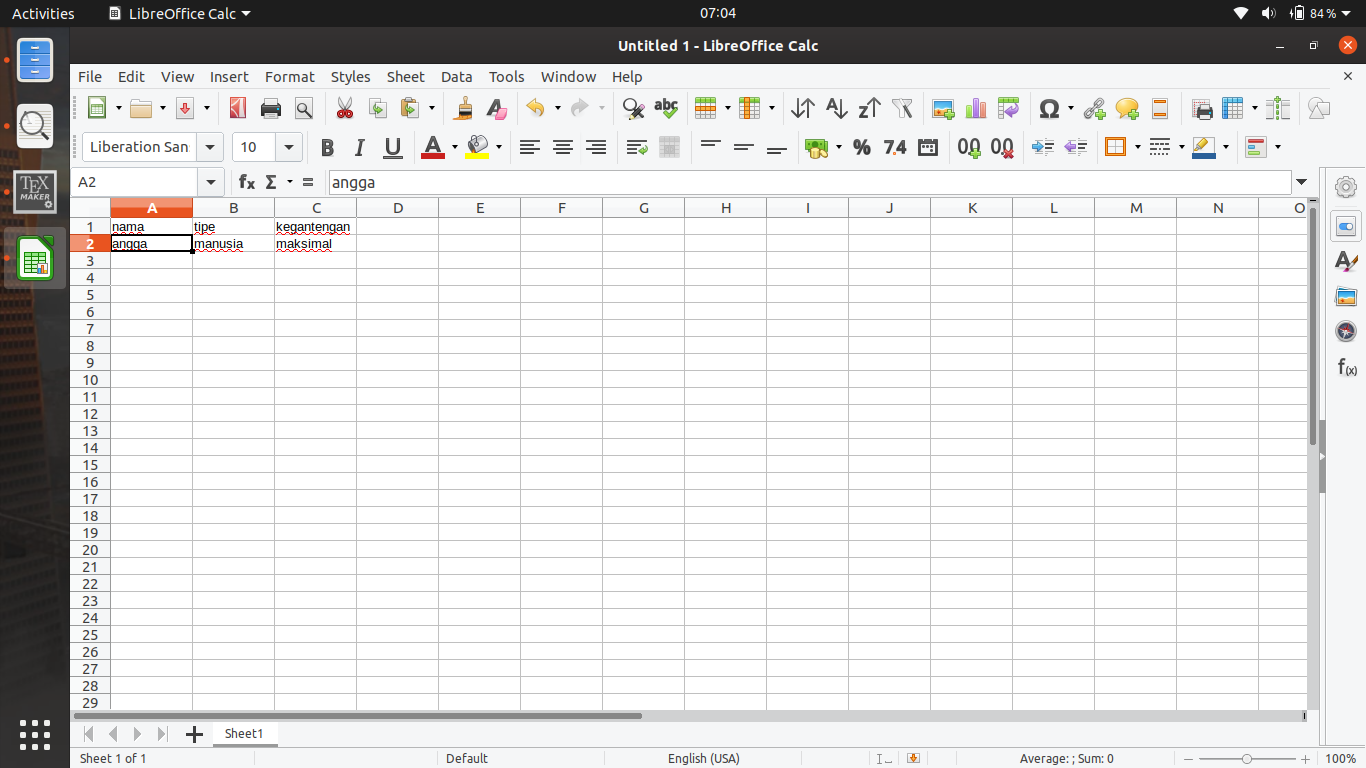
\includegraphics[width=1\textwidth]{figures/wek1.png}
\label{tuliscsv}
\end{figure}
setelah itu kita bisa langsung save as atau export menjadi file csv
\begin{figure}[H]
\centering
\caption{Membuat File CSV}
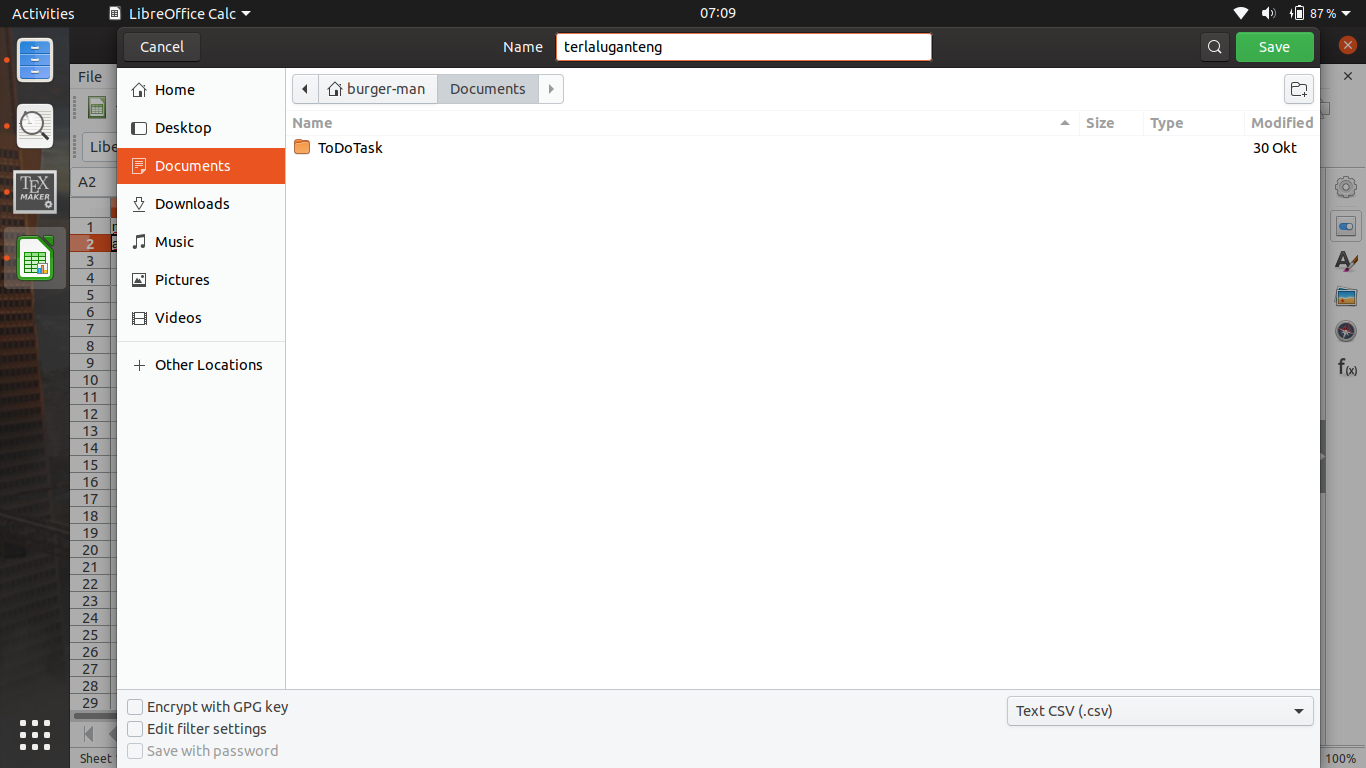
\includegraphics[width=1\textwidth]{figures/wek2.png}
\label{buatcsv}
\end{figure}
cara membacanya adalah tulisan sebelum koma pertama adalah kolom pertama lalu tulisan sebelum koma kedua kolom kedua dan seterusnya.

\subsection{CSV Library}
Library CSV pada python merupakan sebuah package yang dapat digunakan untuk mengolah sebuah file csv mulai dari menulis, mengedit, maupun membaca file csv yang sudah ada. Sehingga programmer dapat dengan mudah mengolah csv nya dengan bahasa pemrograman tanpa harus mengedit dari sebuah aplikasinya.

\subsection{Pandas Library}
Developer bernama Wes McKinney mulai mengerjakan library pandas pada tahun 2008 saat dia masih bekerja di AQR Capital Management. Saat itu AQR membutuhkan sebuah tool yang kencang, dan fleksibel untuk mengerjakan sebuah analisis kuantitatif pada data keuangan. Setelah Wes meninggalkan AQR ada karyawan yang melanjutkan pandas bernama Chang She pada tahun 2012. Pada 2015, pandas disponsori oleh NumFOCUS sebuah lembaga nonprofit di Amerika Serikat.

\subsection{CSV Function}
\begin{enumerate}
\item writer, untuk menulis atau membuat sebuah file csv dengan record didalamnya.
\item reader, untuk membaca semua record yang berada didalam file csv.
\item register dialect, untuk mendaftarkan suatu dialect kedalam sebuah kelas atau subkelas.
\item unregister dialect, untuk menghapus sebuah dialect dari daftar dialect.
\item get dialect, untuk mengambil data dialect dari daftar dialect.
\item list dialect, menampilkan semua daftar dialect yang telah didaftarkan.
\item field size limit, untuk menentukan limit parsing dari sebuah dialect.
\end{enumerate}

\subsection{Pandas Function}
\begin{enumerate}
\item pivot table, untuk membuat sebuah spreadsheet dengan style tabel pivot sebagai DataFrame.
\item melt, mengubah DataFrame dari pivot menjadi format long tabel.
\item pivot, untuk menampilkan data dari index, column, dan nilai tertentu
\end{enumerate}